\documentclass{article}
\usepackage[margin=1.0in]{geometry}
\usepackage{polski}
\usepackage[utf8]{inputenc}
\date\today
\usepackage{amssymb, amsthm, amsmath}
\usepackage{graphicx}

\title{HPC - CUDA}
\author{Tomasz Kępa \\ \texttt{tk359746@students.mimuw.edu.pl}}

%%%% My macros
\newcommand{\todo}[1]{}
\renewcommand{\todo}[1]{\colorbox{yellow}{ \color{red} \textbf{TODO}: {#1}}}

\begin{document}
\maketitle

\section{Struktura plików}
Rozwiązanie podzielone jest na pliki w następujący sposób:
\begin{enumerate}
  \item \emph{astar\_gpu.cu} -- główny moduł zbierający wszystko w całość, parsujacy flagi i uruchamiający odpowiedni wariant zadania
  \item \emph{config.h} -- struktura przechowujące flagi przekazane do programu
  \item \emph{solver.cuh} -- generyczna implementacja algorytmu GA*. 
  			Klasa ta trzyma rozwijane stany i odpowiada za konstruowanie pomocniczych struktur danych. 
  			Tutaj znajduje się też główna pętla algorytmu
  \item Detale związane z konkretnym problemami znajdują się w następujących plikach:
    \begin{enumerate}
      \item \emph{pathfinding.cuh} oraz \emph{pathfinding.cu} -- implementacja problemu \emph{pathfinding}
      \item \emph{slidingpuzzle.cuh} oraz \emph{slidingpuzzle.cu} -- implementacja problemu \emph{sliding puzzle}
    \end{enumerate}
  \item Struktury danych wykorzystywane przez algorytm:
    \begin{enumerate}
      \item \emph{hashtable.cuh} -- tablica hashująca opisana w artykule
      \item \emph{queues.cuh} -- struktura przechowująca zadaną liczbę kolejek o ustalonym maksymalnym rozmiarze
      \item \emph{lock.cuh} -- prosty mutex wykorzysytany do stworzenia sekcji krytycznej "per blok" 
                (jeden z wątków z bloku walczy o locka, w sekcji krytycznej znajduje się cały blok)
    \end{enumerate}
  \item Mniej ważne pliki pomocnicze
    \begin{enumerate}
      \item \emph{errors.h} -- pomocnicze funkcje obsługujące błędy alokacji i błędy zwrócone przez funkcje CUDY
      \item \emph{memory.h} -- pomocnicze funkcje do zwalniania pamięci
    \end{enumerate}
\end{enumerate}

\section{Opis rozwiązania}
Zamknięte stany trzymane są w statycznej tablicy przechowywanej przez klasę \emph{Solver}. 
W celu zaoszczędzenia pamięci, zamiast wskaźników, używane są indeksy poprzednich stanów.
Synchronizacja polega na zwiększaniu przez wątki wartości zmiennej trzymającej następny wolny indeks (za pomocą \emph{atomicAdd})
Typ przechowywanych stanów definiowany jest przez klasy odpowiadające odpowiednim problemom w ich plikach nagłówkowych
(klasy \emph{State} w plikach \emph{pathfinding.cuh} oraz \emph{slidingpuzzle.cuh})

Kolejki mają statyczne rozmiary i jest ich dokładnie tyle samo co wątków. Synchronizacja przebiega w sposób następujący:
\begin{enumerate}
 \item Pobieranie elementu z kolejki -- każdy wątek ma swoją kolejkę i w trakcie wyjmowania elementu kolejki jest zapewnione, 
          że żaden inny wątek w tym samym czasie nie będzie próbował ani nic wkładać ani wyciągać z kolejki
 \item Dodawanie elementu do kolejki -- tutaj zapewniam synchronizację "per blok", czyli w momencie gdy piszę coś do kolejek to pracuje w tym czasie
          tylko jeden blok, a każdy wątek wpisuje coś wyłącznie do kolejek odpowiadających wątkom o tym samym indeksie w bloku, 
          tak aby nie była konieczna synchronizacja pomiędzy wątkami w tym samym bloku
\end{enumerate}

Algorytm wykonywany jest w wyraźnych krokach, tak jak były opisane w artykule. Wszystkie wątki zaczynają krok razem i kończą go razem. Dodatkowe 
synchronizacje opisane są w poszczególnych punktach. W skrócie fazy wykonania algorytmu:
\begin{enumerate}
\item Extract -- każdy wątek wyciąga jeden element ze swojej kolejki. W tym etapie wątek przygotowuje sobie miejsce w głównej tablicy stanów
        na zapisanie swoich nowych stanów (przez użycie \emph{atomicAdd})
\item Expand -- każdy wątek ekspanduje swój stan i sprawdza, czy taki 
        lub lepszy (czyli o tym samym \emph{node} ale lepszej wartości \emph{g}) jest już w tablicy. 
        Jeśli nie to wpisuje nowy stan do tablicy rozwiniętych stanów. 
        Jeśli już znany jest lepszy stan to ten stan jest pomijany. Przygotowane miejsce nie marnuje się 
        -- nadal może być użyte przez ten wątek w późniejszym kroku algorytmu.
        Wartości \emph{f} i \emph{g} liczone są już w tym etapie. 
\item Deduplicate -- etap ten również wykonywany jest bez dodatkowych synchronizacji ze względu na to, że pozwala na to nasza tablica hashująca.
        Jeśli jakiś stan zostanie zdeduplikowany dopiero na tym etapie (bo inny wątek dopisał w międzyczasie lepszy stan) 
        to już nie zwalniam pamięci tego stanu, tylko oznaczam go jako usunięty.
\item Compute -- ten etap wykonywany jest w mojej implementacji w trakcie etapu Expand, 
        ze względu na to, że używane są proste heurystyki i niewiele by pomogło ich liczenie
        dopiero po deduplikacji. Dodatkowo, etapy po deduplikacji są u mnie synchronizowane "per blok", przez co tym bardziej korzystne jest policzyć
        te wartości od razu
\item Push-Back -- W tym etapie następuje synchronizacja "per blok" (aktywny jest tylko jeden blok na raz). 
        Wszystkie wątki z bloku zbierają w jednej tablicy indeksy nowo rozwiniętych stanów, a następnie wpisują
        stany do odpowiednich kolejek tak jak opisano wcześniej.
\item Check Final Conditions -- jest to etap nie nazwany explicite w artykule. Podzielony jest na dwa podetapy:
  \begin{enumerate}
    \item sprawdzenie czy znaleziono już ścieżkę -- w trakcie ekspansji stanów każdy wątek zapisuje najlepszy napotkany przez siebie stan końcowy.
           Dopiero tutaj natomiast następuje zebranie tych wyników najpierw w najlepszy stan "per blok",
            a następnie najlepszy globalny stan. Następnie, jeśli spełniony jest
           warunek końcowy (wszystkie stany w kolejkach mają nie lepsze wartości \emph{f}) to algorytm kończy działanie
    \item sprawdzenie czy nie przeszukano wszystkich stanów -- jeden z wątków sprawdza rozmiary wszystkich kolejek. Jeśli wszystkie
           kolejki są puste to rozwiązanie nie istnieje. Pętla ta jest wykonywana przez tylko jeden wątek ponieważ i tak przez większość czasu
           wszystkie kolejki są niepuste
  \end{enumerate}
Na tym etapie synchronizuję wszystkie wątki, do czego używam funkcjonalności "Cooperative Groups".
\end{enumerate}

\section{Optymalizacje}
\subsection{Pamięć}
Za każdym razem staram się zaalokować najwięcej pamieci jak tylko możliwe, ponieważ nie wiadomo ile stanów potrzeba rozwinąć przed znalezieniem
rozwiązania. Możliwe byłoby użycie streamów i alokowanie np. tablicy stanów kawałkami, ale nie starczyło mi czasu aby to zaimplementować. 
Inna możliwość, której nie sprawdziłem a mogłaby pomóc to użycie "Texture memory" do problemu \emph{pathfinding}.

Ważną rzeczą związaną z pamięcią, jaką zaaplikowałem, to użycie "Constant memory" to elementów konfiguracji. W obu przypadkach
chodzi o końcowe konfiguracje, z którymi to bardzo często trzeba się porównywać.

W przypadku problemu \emph{sliding puzzle} mam mapę "liczba -> pozycja", która służy do liczenia heurystyki. 
Ona również trzymana jest w "Constant memory".

\subsection{Obliczenia}
W przypadku algorytmu GA* bardzo ważny okazuje się trade-off miedzy możliwością rozwijania dużej liczby stanów na raz a zużywaną pamięcią.
Ustawione w kodzie ilości wątków i rozmiary struktur dobrane są dla karty GTX1060 (6Gb ram, 10SM).

Wyniki profilowania wskazują niestety na małe wykorzystanie potencjału karty (zob. zrzuty). 
Wskazuje to na niewykorzystane możliwości optymalizacji.

\begin{figure}[htb]
        \center{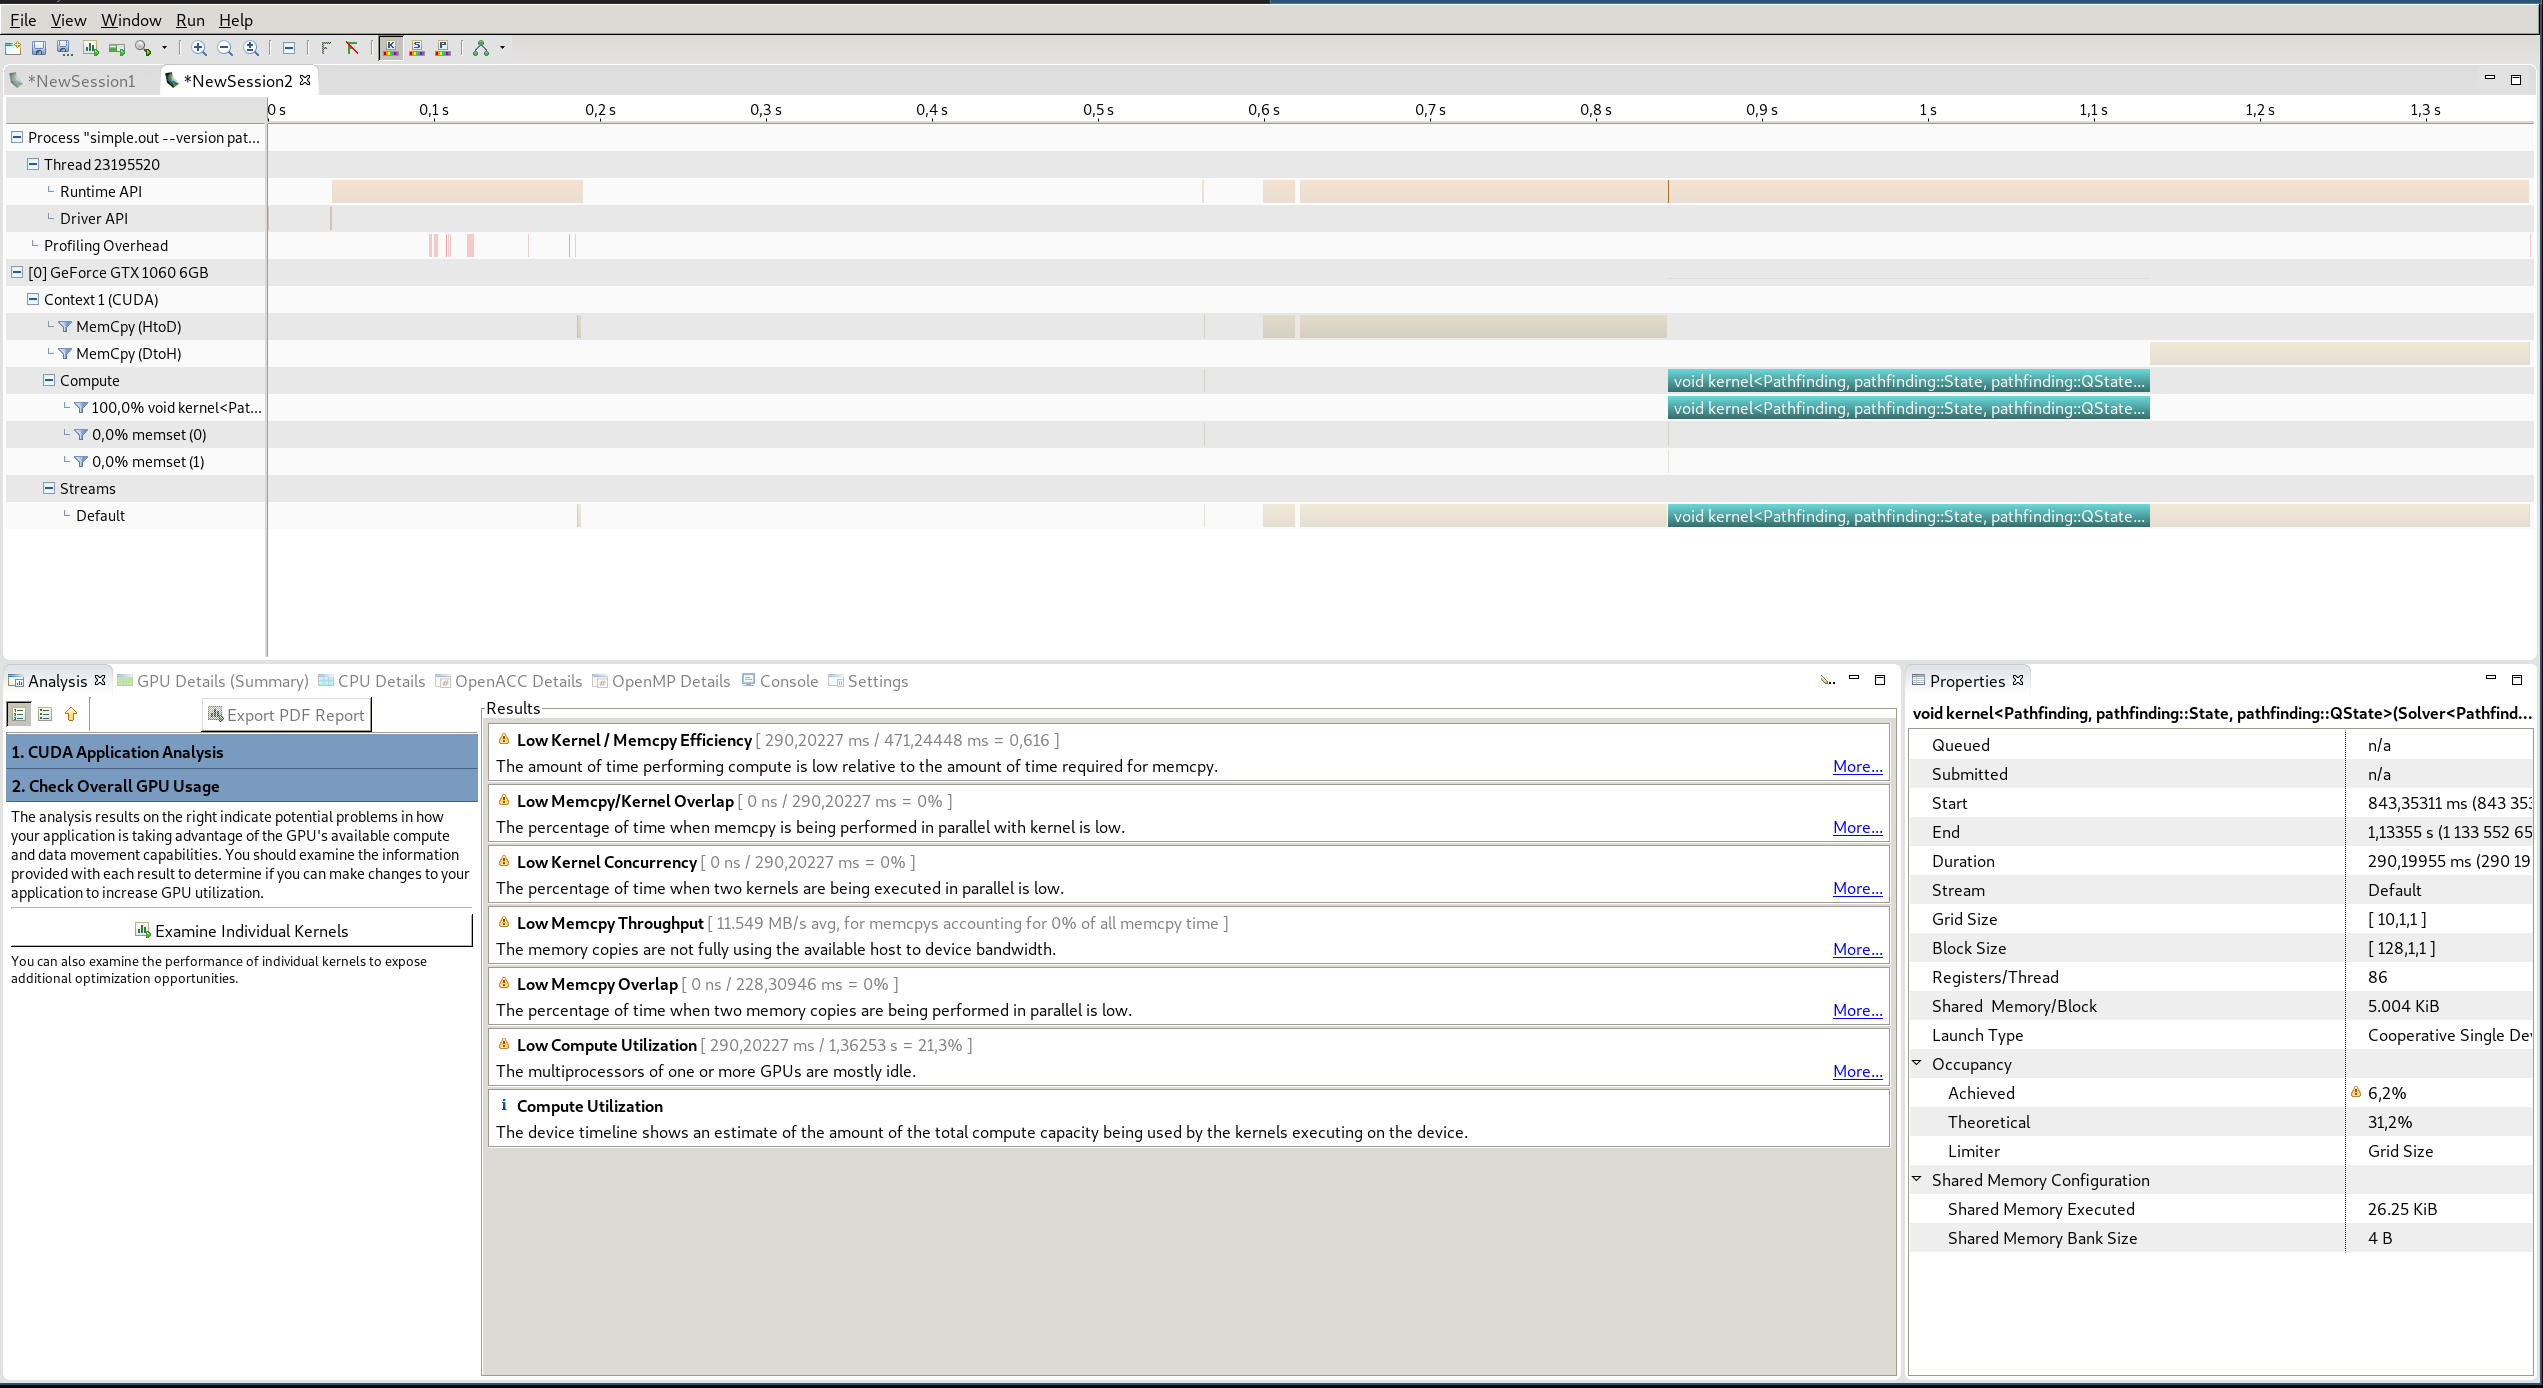
\includegraphics[width=\textwidth]{img/pathfinding_simple_1000_util}}
        \caption{\label{fig:path} Wykorzystanie karty. Problem \emph{pathfinding}, plansza 1000 x 1000}
\end{figure}
    
\begin{figure}[htb]
        \center{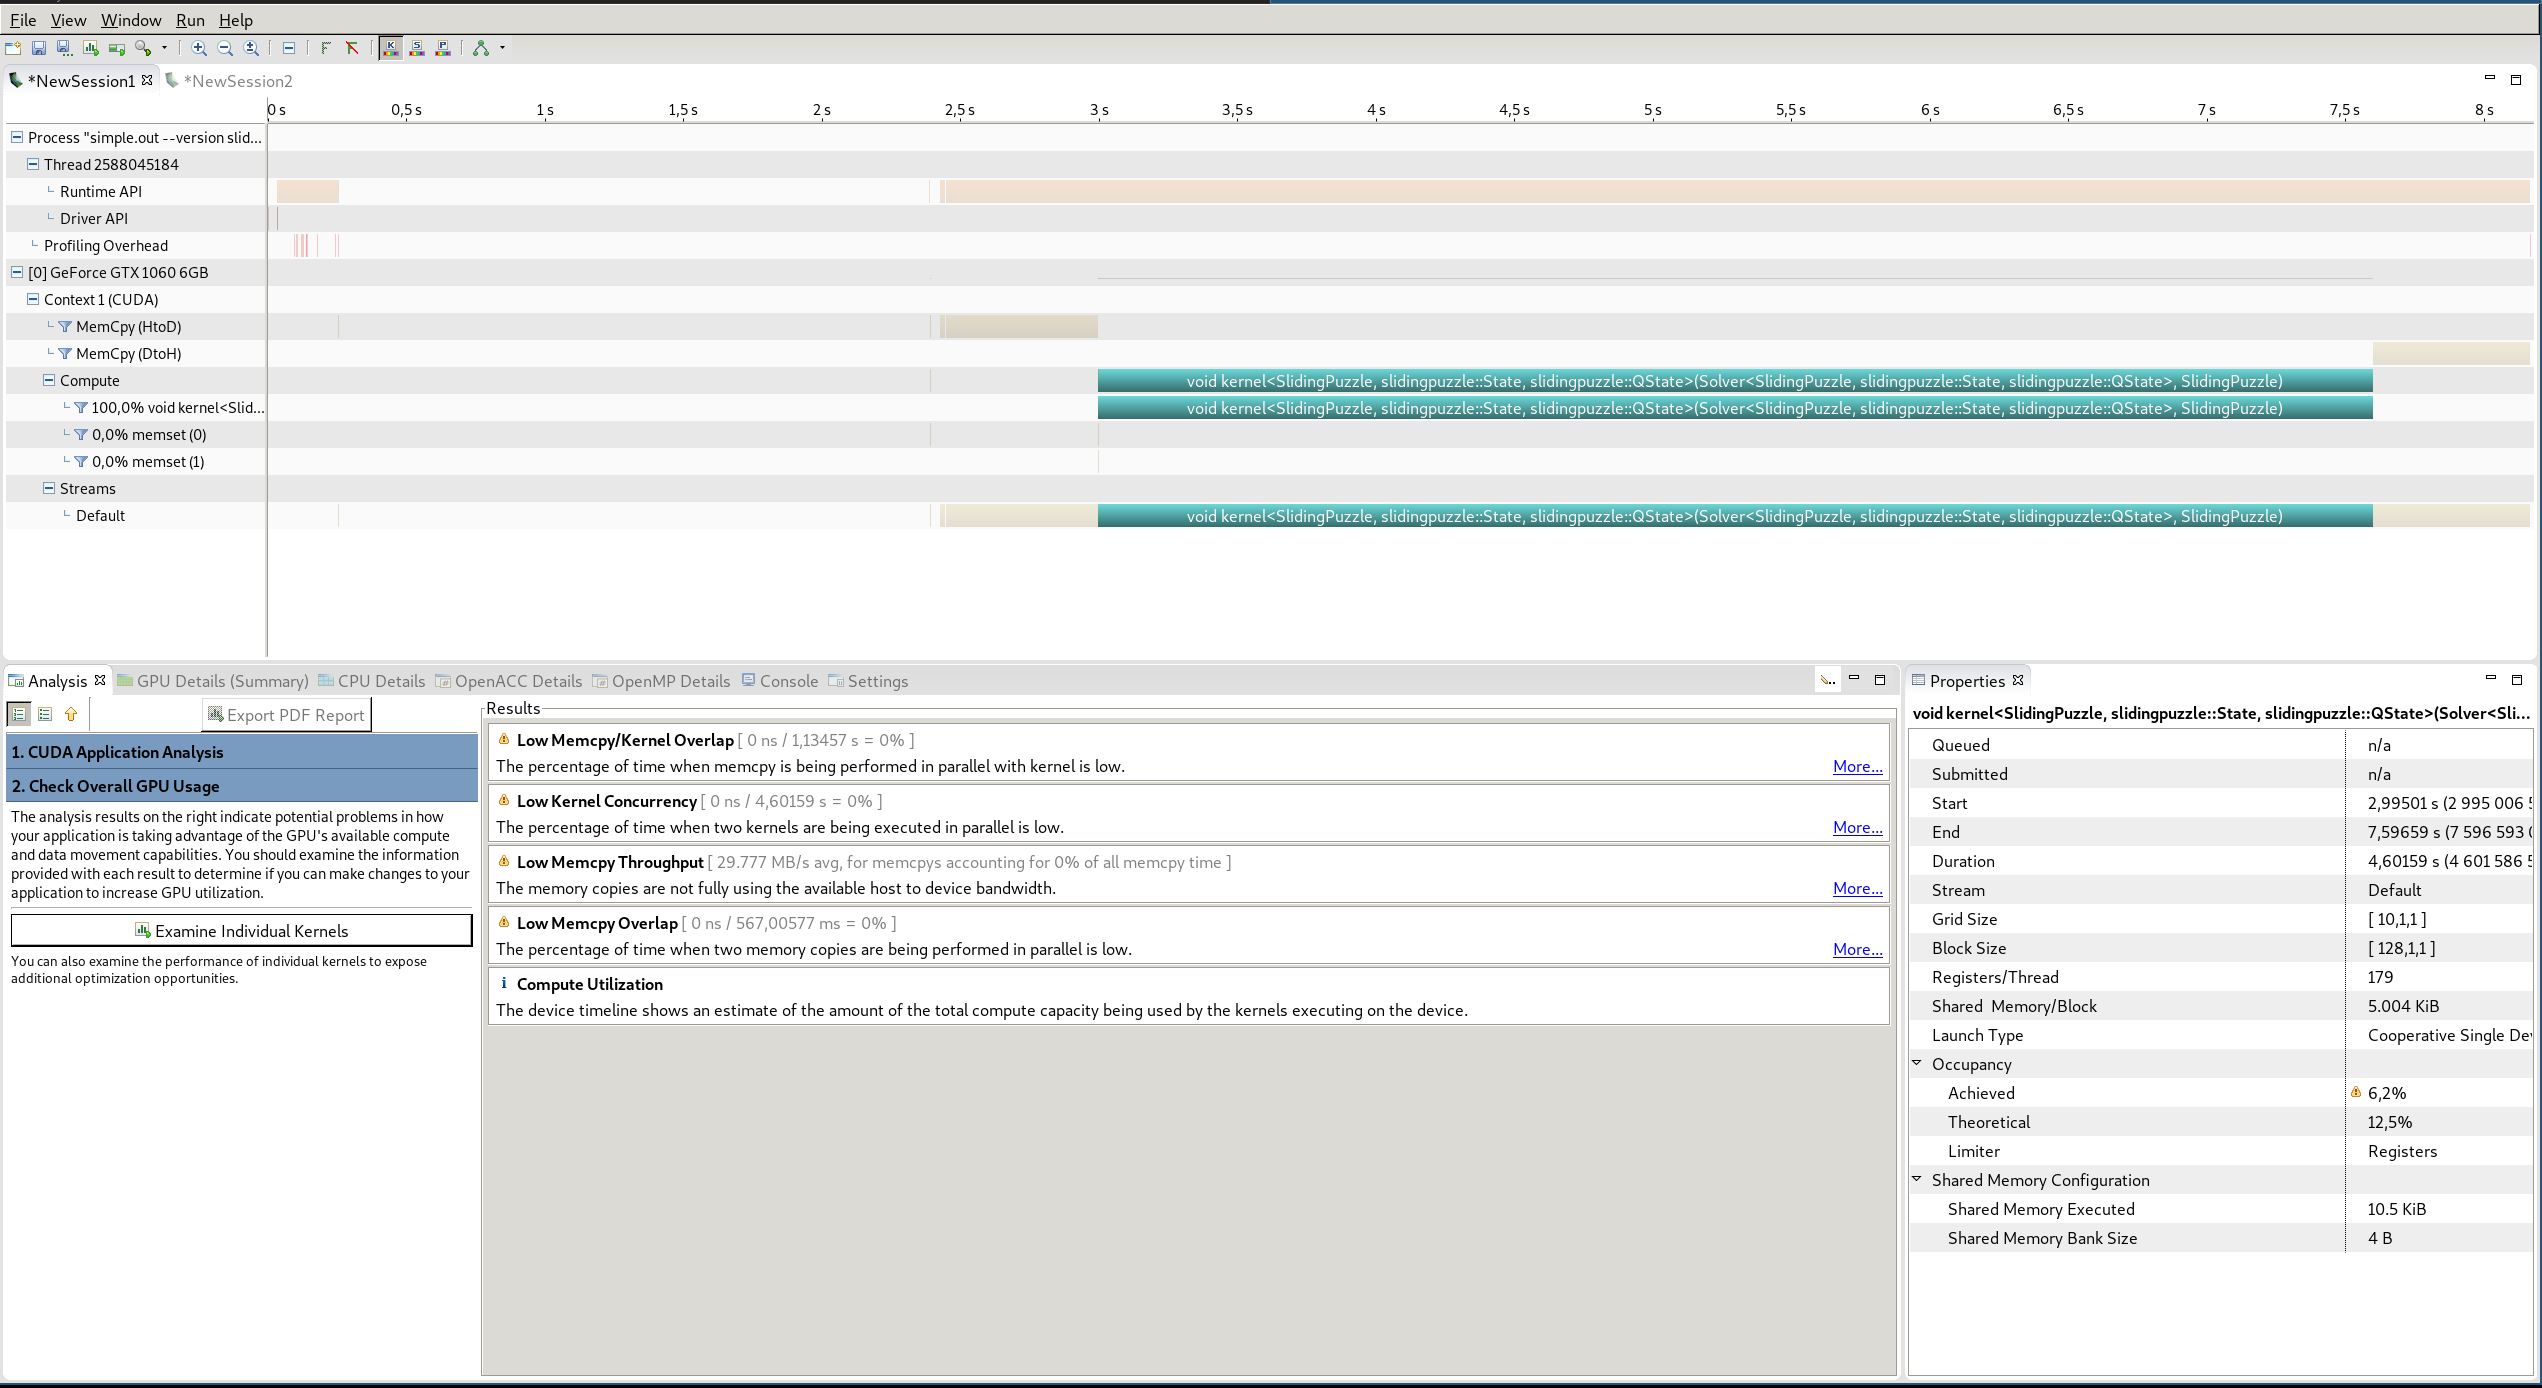
\includegraphics[width=\textwidth]{img/slidingpuzzle_30}}
        \caption{\label{fig:sliding} Wykorzystanie karty. Problem \emph{sliding puzzle}, ścieżka długości 30 ruchów}
\end{figure}

\section{Heurystyki}
\subsection{Pathfinding}
W tym przypadku zaproponowana w zadaniu metryka jest niepoprawna, ponieważ dopuszczamy ruchy "na ukos", przez co bardzo łatwo
o przypadki, kiedy odległość policzona przez heurystykę jest większa niż rzeczywista odległość.

Heurystyka zaimplementowana przeze mnie, pozbawiona powyższego błędu, jest następująca:
$$h= \max(|x_1 - x_2|, |y_1 - y_2|)$$

\subsection{Sliding puzzle}
Tutaj zaproponowana heurystyka jest w porządku, trzeba tylko pamiętać, żeby nie doliczać odległości pustego fragmentu.

\end{document}